In Hogwarts, everything is based on wizardry and spells: for this reason the wand, together with protective jewelry, will play an important role in combat, enhancing the magical capabilities of our characters in different ways.

The wand is the most important tool in a wizard's life: inner magical power is channeled through it and it can cast any kind of spell. Each wand is made of wood and contains an enchanted core, a special material usually coming from magical creatures.
\centeredgraphicssize{../Pictures/Gameplay/Items/Wand_picture.jpg}{5cm}
There are several types of wand wood and cores, which will alter and enhance the capabilities of the wielder.

\paragraph{Wood} 

The wood will grant a bonus to its particular category of spells: \\

\begin{tabular}{ m{4cm}m{3cm}m{6cm} } 
	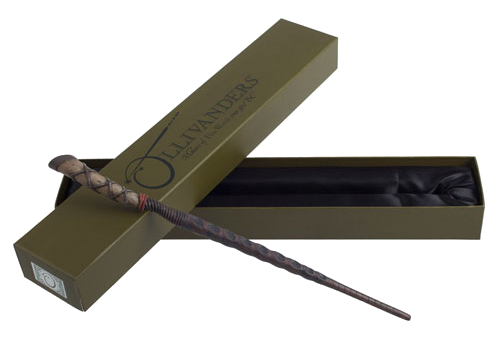
\includegraphics[width=4cm]{../Pictures/Gameplay/Items/Wearables/Wand/Wood/Holly_wood_picture.png} & \textbf{Holly} & Holly will boost defensive spells, naturally meant for casters who think that a good defense is the best offense. \\ 
	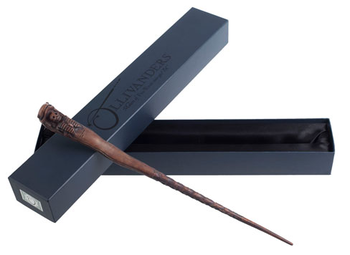
\includegraphics[width=4cm]{../Pictures/Gameplay/Items/Wearables/Wand/Wood/Alder_wood_picture.png} & \textbf{Alder} & Alder will boost buff spells, aiding mages who seek to help and empower others. \\ 
	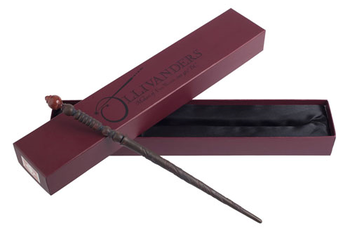
\includegraphics[width=4cm]{../Pictures/Gameplay/Items/Wearables/Wand/Wood/Cedar_wood_picture.png} & \textbf{Cedar} & Cedar will boost debuff spells, perfect for wizards who prefer to weaken their enemies before striking.  \\ 
	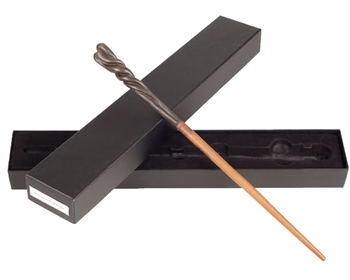
\includegraphics[width=4cm]{../Pictures/Gameplay/Items/Wearables/Wand/Wood/Cherry_wood_picture.png} & \textbf{Cherry} & Cherry will boost attack spells, favored by sorcerers who follow the rule "strike first, strike hard". \\ 
	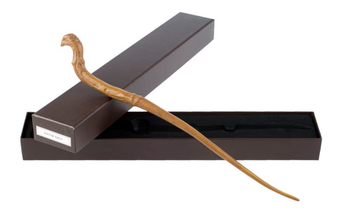
\includegraphics[width=4cm]{../Pictures/Gameplay/Items/Wearables/Wand/Wood/Pine_wood_picture.png} & \textbf{Pine} & Pine will boost utility spells, preferred by creative enchanters and out-of-the-box thinkers. \\ 
\end{tabular}
\pagebreak 
\begin{itemize}
    \item The bonus for non-Utility category will make spells of that category cast as 1 level higher (if applicable).
    \item The bonus for Utility category will grant an extra spell slot reserved to Utility spells for each spell level the character has access to.
\end{itemize}

\clearpage